\documentclass[conference,letterpaper]{IEEEtran}
\IEEEoverridecommandlockouts

\usepackage{amsmath,amssymb,amsfonts}
\usepackage{graphicx}
\usepackage{textcomp}
\usepackage[OT1]{fontenc}
\usepackage{pifont}
\usepackage{multirow}
\usepackage{threeparttable}
\usepackage{booktabs}% 
\usepackage{gensymb}
\newcommand{\tabitem}{~~\llap{\textbullet}~~}

\def\BibTeX{{\rm B\kern-.05em{\sc i\kern-.025em b}\kern-.08em
T\kern-.1667em\lower.7ex\hbox{E}\kern-.125emX}}
\begin{document}
\bstctlcite{IEEEexample:BSTcontrol}

\title{The Impact of Inaccuracies in Thermostats: An Energy and Cost Analysis}
%
\author{
\IEEEauthorblockN{
Anvitha Ramachandran,
Emily Laus,
Frank Catalano,
Kushagra Srivastava
}
\IEEEauthorblockA{
\textit{Integrated Concentration in Science Program at UMass Amherst}\\
Amherst, MA \\}
}

\maketitle

\begin{abstract}
Heating, Ventilation, and Air Conditioning (HVAC) systems are essential for indoor comfort, but the systems account for more than $40\%$ of energy consumption in a typical industrial building. What's more, this energy consumption is dependent on the readings and inputs of building thermostats, meaning that energy can easily be wasted if the thermostats are not accurate and precise. This report details the impact of inaccurate thermostats on the energy and money waste from a room. Through a simulation of heat flow and energy consumption, we aim to quantify these impacts and compare the financial cost of retrofitting a building to the savings and decrease in energy consumption. The simulation is verified by previous experiments related to heat and energy consumption, and the experiment is applied to UMass's W.E.B. DuBois Library.

\end{abstract}

\begin{IEEEkeywords}
thermostats, energy consumption, HVAC, simulation
\end{IEEEkeywords}

\section{Introduction}
\label{sec:Introduction}
In total, $3.9\%$ of global greenhouse gas emissions and 
10\% of global electricity usage overall originate from air conditioning systems. According to a report by the International Energy Agency (IEA), targeting specific inefficiencies of air conditioning systems is paramount to reducing the total energy consumption of buildings, since air conditioning contributes to 
20\%  of office building electricity use \cite{IEA_Future} . Woods et al. discusses the impact of humidity on the energy wasted and emissions produced by air conditioning systems, stating that "managing humidity in the building environment is as important as controlling temperature" \cite{woods_humiditys_2022}, and that appropriate control of both is necessary to minimize excess use of energy and refrigerant materials for air conditioning and reduce costs of HVAC systems to improve accessibility. Therefore, similar analysis on the impact of inaccurate thermostats on control mechanisms would provide a similar benefit to the Woods et al. paper. 

Our research aims to answer the question "What excess energy and financial costs result from inaccurate thermostats installed in a room?".  Section \ref{sec:Background} discusses the previous studies of HVAC design principles, sources of energy inefficiency, and models for simulating thermostat control, all of which inspired the design and structure for our simulation. The principles that define the simulation's design are expressed in Section \ref{sec:Methods}, describing the hybrid simulation architecture inspired by the background readings. Section \ref{sec:Results} defines how we will evaluate and interpret the results of our simulation. Lastly, Section \ref{sec:Conclusion} details elements of the research that could be further developed in future research.

\section{Background}
The background research regarding designing such a simulation can be split into three fundamental categories: designing an HVAC system, highlighting its inefficiencies and how those inefficiencies can be modelled so their propagating effects through the system can be analyzed.
\label{sec:Background}
\subsection{Measures for Designing HVAC Systems}
In order to develop a representative simulation for determining the impact of inaccurate thermostats on the controls for maintaining the temperature of a room, we had to analyze what fundamental features for an HVAC system would go into a simulation of the controls. For example, in a report by Philip Luu for Texas Instruments \cite{Luu2021} regarding the use of one of their sensors for an HVAC system, they describe the general structure of an HVAC system. This is essentially a thermostat with sensors and user control as well as a central controller for controlling the behavior of the air in the room. After detecting a change in the controller signal value [which occur because of changes in the temperature of the mixed-air chamber or changes in the desired temperature], air must be brought into the mixed air chamber to be treated to flow through the supply duct. For enthalpy economization, sensors are placed in the outdoor and return air ducts to determine the air with lower enthalpy to be brought in to the mixed air duct and then heating/cooling coils treat it to be the appropriate temperature and be blown through the room. 

The study from Asim et al. about the sustainability of HVAC units \cite{ijerph19021016} corroborates this, describing a similar valve structure with heating and cooling coils to modify the temperature of the air. It suggested a variety of modification methods, each affecting separate parts of the system, which implies a modular construction to target sore points. It describes targeting a sore point via retrofiting as upgrading "mechanical systems" such as the thermostats and control algorithms in older buildings for retro fitting, and "establishments of the relationship between the investment of retrofitting and the sustainability performance", and a modular configuration would be conducive to drawing such comparisons for retrofitting prior to evaluating their benefits.

\subsection{Sources for Inefficiency in HVAC Systems}
To build an accurate simulation, we need to study major sources of inefficiency in HVAC systems, and how they may affect current room temperature and energy consumption. Sudhi Sinha, Vice President of Johnson Controls, states in a study that a temperature misreading of about 0.5 degrees Celsius can lead to a higher energy consumption of about 17\% \cite{Sinha2014}. In the case of a typical 100,000 sq. ft building, this would result in a financial excess of \$29,000 each year.

Moreover, older thermostats which use a Bimetallic Strip are also prone to furthermore inaccuracies. These thermostats experience Wear and Tear over time, i.e., their temperature reading accuracy diminishes over time due to the stress induced on the bimetallic strip. This is a phenomenon known as "Sensor Drift", and as a result, such thermostats usually need calibration done by a professional every 2 years or so. Sensor Drift can account for inaccurate readings ranging from 3-5 degrees Celsius in the short term, and up to 5-10 degree Celsius long term, thus compounding the excess costs mentioned earlier \cite{Luu2021}. 

Even though newer thermostats can mitigate Sensor Drift by using digital sensors, the newer enthalpy-based HVAC measurement systems also account for room humidity. While this measure can prove to be cost-saving, it usually runs the risk of humidity inaccuracies leading to similar cost increases \cite{Luu2021}. 

Furthermore, a research study conducted by the Denmark Technical University also showcased how important the placement of a thermostat can be in determining the accuracy of the sensor \cite{madsen1990a}. The Research took 3 different room settings, including a Living Room, The Danish Parliament, and The Royal Theater at Denmark. Different locations were tested for the thermostats in each setting, and the results found that Thermostats are most accurate in central locations of any room, and there was a discrepancy of about +/- 1-2 degrees Celsius whenever the thermostats were in any corner positions or the walls. 

The proximity of the sensors from direct sunlight, HVAC Vents, and sheltered areas of the room also lead to inaccuracy. Based on the Johnson Controls study mentioned above, we can infer that just the positioning of the thermostats may account for a high cost increase. Other factors may also include room materials, insulation, height of the thermostat sensor, and enclosures around the thermostat sensors.

Another study conducted by the University of California at Davis also suggests some uncontrollable factors that may go into determining the efficiency of Thermostats. These may include Human Contributors (room occupants, technicians, building owners, etc.), amount/quality of HVAC maintenance, and general functioning of the HVAC System (surface temperatures of HVAC systems, pipe maintenance, pressure of different gases in the system, etc.) \cite{Heinemeier2012UncertaintiesIA}. While we may not be able to include such factors due to a time constraint, and due to the general nature of such problems, it is important to keep in mind such factors which may contribute towards inaccurate temperature readings. 

Overall, the factors mentioned above play a big role in temperature reading accuracy, which further plays a big role in determining excess energy and cost usage of such systems.

\subsection{Models for Simulating Thermostat Control}
To make the simulation modular for the reasons demonstrated in earlier sections, we must study the models that are used for various components of the HVAC system, such as those of the heating and cooling coils, the various types of valves, and the design of how those are linked for a singular room. Since the research question aims to understand the effect of thermostat placement, quantity and accuracy on control models, we will be focusing more of our care on exploring the variety of the controller and the thermostat models to address these qualities of the HVAC system. 

An understanding of the mental models for thermostat control that are commonly seen in literature is fundamental to the design of a model that couples with the rest of the HVAC system well, which is provided by Revell et al. in their case study of such models, a lens into the state of the field and what types of models exist for such a control system \cite{revell_case_2014}. 

As a system that people use en masse, it makes sense to understand how human behavior impacts the energy efficiency of an HVAC system, especially with respect to thermostat control, since misuse of thermostats [i.e., changing their programmed temperature too rapidly or too often] can be an issue if the thermostat allows for that type of programmable control. The paper from Pritoni et al. on this topic \cite{pritoni_energy_2015} suggests the idea of internet-connected smart thermostats and a control system for more transparency of how the thermostat is being changed so that people's behavior can be verified. Public buildings with a large number of patrons would likely disable this programmability feature, but studying the energy impact of such an adverse switching state would help us model a thermostat with less hysteresis in its design, which we know would be adverse from the Revell et al. paper's models mentioning so, but it would quantify the waste due to a lack of appropriate hysteresis in the system.  

To simulate the physical phenomena that occur in an HVAC system, the air flow within the ducts is paramount to demonstrate the interactions of the system that are done to maintain the temperature value according to the thermostat's settings. In Alashme et al.'s paper \textit{A virtual thermostat for local temperature control} \cite{alhashme_virtual_2016}, point-based ideal heating is maintained by using fluid dynamics to determine how the air flows through vents to sustain a certain value at specific regions of the room.  

\section{Methods}
\label{sec:Methods}
In order to analyze the consequences of inaccurate thermostats, we simulate a room that has a traditional HVAC system with the thermostats in Section \ref{sec:Background}. The system will be designed with a hybrid model, i.e. one that uses the techniques expressed in Section \ref{sec:Background} to create a modular system that can be generalized to any rectangular room. 
% \subsection{Thermodynamic Assumptions}
% \begin{figure}[ht!]
% \centering
% 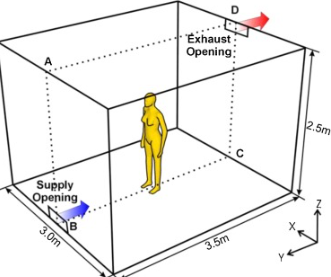
\includegraphics[scale=1.25]{room.png}
% \caption{Ideal room structure, for Thermodynamic Assumption 1.}
% \centering
% \end{figure}
\subsection{Thermodynamic Assumptions}
\begin{figure}[ht!]
\centering
%\begin{subfigure}{\linewidth}
\centering
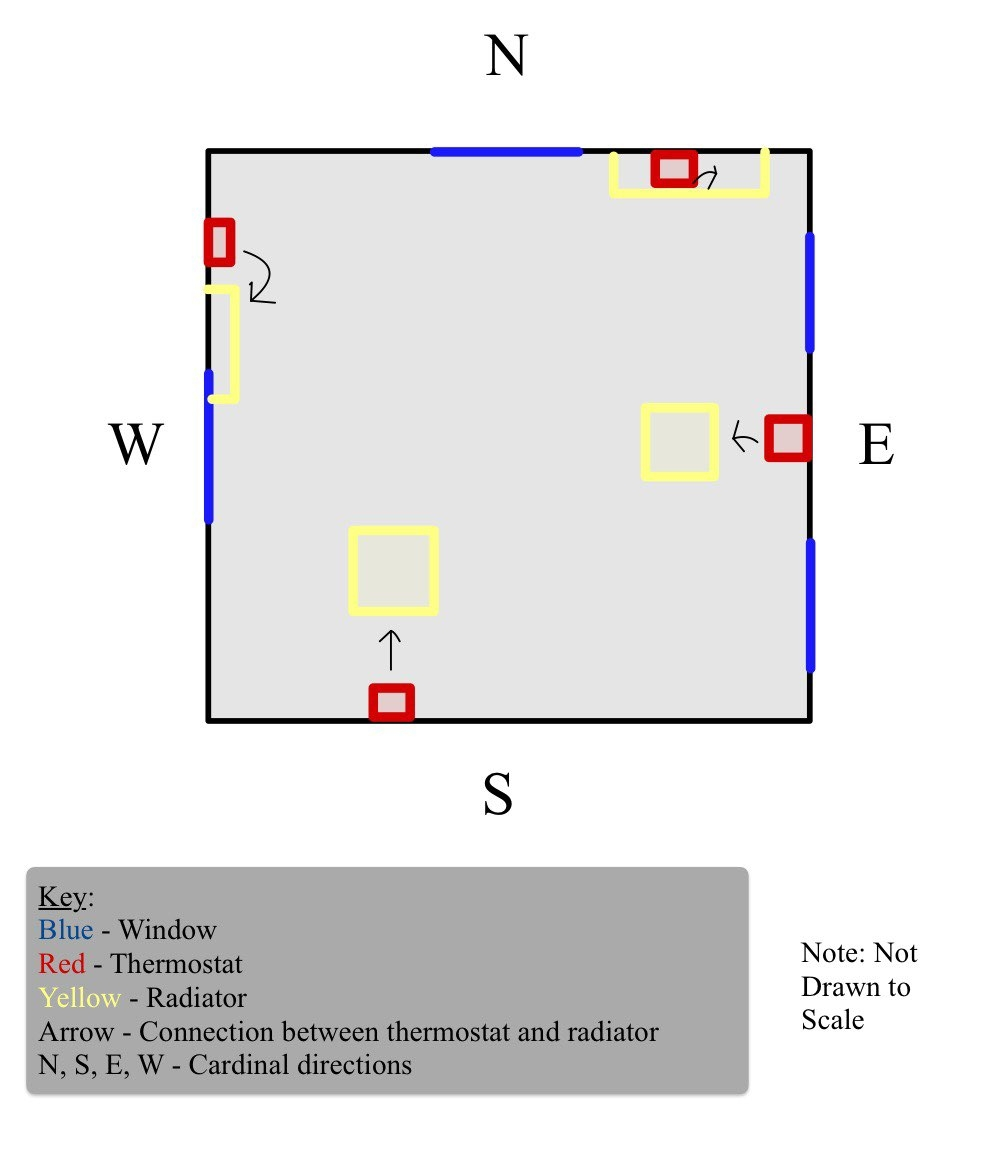
\includegraphics[scale=0.2]{room_2.jpg}
%\end{subfigure}
%\begin{subfigure}{\linewidth}
\centering
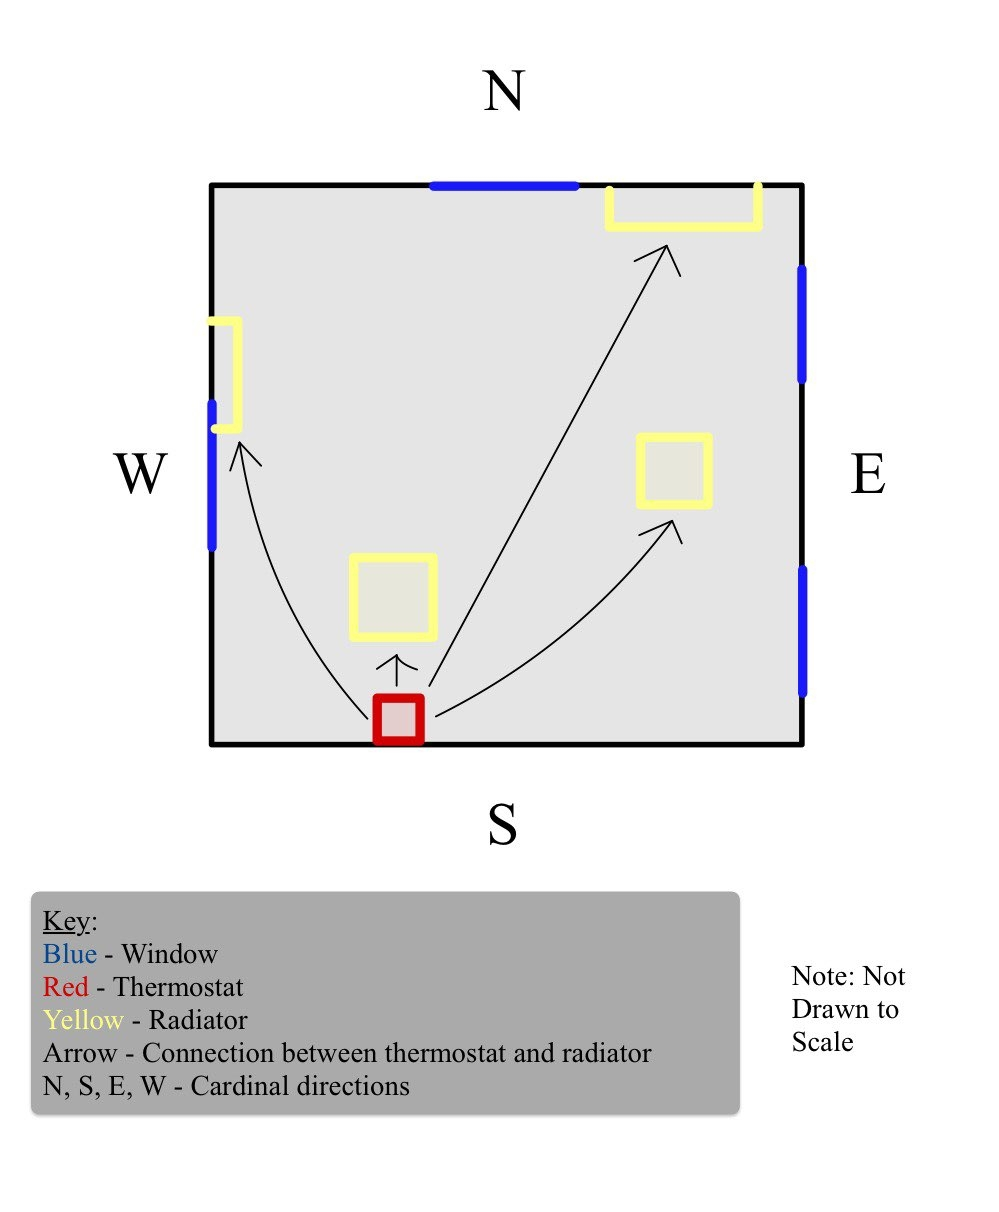
\includegraphics[scale=0.2]{room_3.jpg}
%\end{subfigure}
\caption{Ideal room structure, for Thermodynamic Assumption 1.}
\label{fig:thermo_assumptions}
\end{figure}
To maximize the usability of our simulation while preventing over-complication for construction, we apply some assumptions to the conditions of the room we model. Our assumptions are as follows:

\begin{enumerate}
    \item The shape of the room that we model is a rectangular prism. This can characterize an approximate average shape of a room, especially compared to the rooms that we will be evaluating to verify the model [elaborated on in Section \ref{sec:Results}]. 
    \begin{itemize}
        \item The length and width of the room will be user inputs, as will relevant constants (i.e., insulation value) regarding the walls, floor and ceiling.
    \end{itemize}
    \item The walls, floor, and ceiling are a consistent, homogeneous material.
    \begin{itemize}
        \item These outer surfaces can be different materials and have different types of insulation (see the User-Adjustable Parameters [Inputs] section), but the material and insulation inputs will apply to the entire surface (wall, ceiling, or floor).
    \end{itemize}
        \item The desired temperature in the room is constant and even throughout the room. (We do not account for a preference in different temperatures throughout the same room.)
    \begin{itemize}
        \item The thermostat can be lowered to no lower than 50$\degree$F. Colder temperatures can lead to frozen pipes and infrastructure damage. \cite{constellation}
        \item The thermostat can be raised to no higher than 80$\degree$F. Warmer temperatures can promote mold growth and unhealthy conditions for people to reside in.
    \end{itemize}
    \item The modeled room has no doors or openings other than closed windows, to minimize the interference in the room's heating due to the airflow of another space.
    \begin{itemize}
        \item All windows have the same dimensions.
    \end{itemize}
    \item The only direct source of heating or cooling in the room  comes from the radiators in the room, which expel hot or cold air to  aid the room in reaching its desired temperature.
    \begin{itemize}
        \item The sun can also change the thermal environment of the room, but it is considered an indirect source of thermal change since it is outside of the room.
        \item No systems designed to supplement an HVAC system (e.g., ground-source heating and cooling) are implemented in this room.
        \item All radiators have the same dimensions.
    \end{itemize}
    \item The airflow from the radiators is a constant velocity and either travels completely upwards (if the radiator is against the wall on the floor) or completely downwards (if the radiator is on the ceiling).
    \item The occupancy of the room is negligible to its heat modeling, so we can approximate as if no people are in the room.
    \item The perpetuation of the sun is constant, meaning that we ignore the existence of clouds in the sky.
    \begin{itemize}
        \item The sun's position can be inputted by the user, as elaborated on in section \ref{sec:Parameters}.
    \end{itemize}
    \item The temperature outside of the room is constant and the exterior wind is negligible to the room's heating.
    \item If the outdoor temperature is below freezing temperature (32$\degree$F), the change in the air's properties outside of the room (e.g., humidity, viscosity, etc.) will not have an effect on the air inside of the room.
    \item  The circulation of air in and out of the room (i.e., vents carrying the air throughout the building to keep the air fresh) is negligible to the room's heating.
    \item One thermostat can control multiple radiators, but one radiator can only be controlled by one thermostat.
    \begin{itemize}
        \item Which thermostat controls a desired radiator can be input by the user.
    \end{itemize}
    \item When the desired temperature of the room (based on the thermostat's input) is different than the perceived real temperature of the room (accounting for the inaccuracy of the thermostat), the HVAC system will aim to obtain the desired temperature for the room within 10 minutes. By setting this time range, we aim to prevent any sudden change in energy input for the HVAC system so that there is no "spike." (For instance, if the HVAC system attempted to heat/cool the room as fast as possible, the room would likely experience a sudden blast of air that would be impractical and expensive.) At the same time, by setting a limit on how long it can take for the room to reach its desired temperature, any occupants would not have to be uncomfortable for too long (assuming that the thermostat is accurate).
\end{enumerate}
\subsection{User-Adjustable Parameters [Inputs]}
\label{sec:Parameters}
The following are the inputs that the user can alter from our simulation, based on Figure 1.

\begin{enumerate}
    \item Preferred temperature units.
    \begin{enumerate}
        \item Fahrenheit ($\degree$F)
        \item Celsius ($\degree$C)
    \end{enumerate}
    \item Desired room temperature.
    \begin{enumerate}
        \item Default: 70$\degree$F
        \item Minimum: 50$\degree$F
        \item Maximum: 80$\degree$F
    \end{enumerate}
    \item Thermostat specifications.
    \begin{enumerate}
        \item Number of thermostats
        \item Placement of each thermostat (only allowed on a wall)
        \item Error of each thermostat (in number of degrees $\degree$F or $\degree$C above or below the desired temperature)
    \end{enumerate}
    \item Window specifications.
    \begin{enumerate}
        \item Number of windows
        \item Placement of each window (only allowed on a wall)
        \item Insulation value
    \end{enumerate}
    \item Radiator specifications.
    \begin{enumerate}
        \item Number of radiators
        \item Placement of each radiator (allowed on a wall or ceiling)
        \item Air Flux (how much air enters the room from each radiator over time)
    \end{enumerate}
    \item Wall specifications.
    \begin{enumerate}
        \item Material (e.g., wood, brick, cement, etc.)
        \item Insulation (e.g., solid wall, insulation filling, hollow wall, etc.)
    \end{enumerate}
    \item Thermostat-Radiator Control Ratio.
    \begin{enumerate}
        \item One thermostat controls all radiators in the room
        \item One thermostat controls one radiator (user chooses which radiator)
    \end{enumerate}
    \item Heating and Cooling Capabilities.
    \begin{enumerate}
        \item Both heating and cooling (the HVAC system can perform either at any time)
        \item Only heating (the HVAC system can only heat the room or remain idle)
        \item Only cooling (the HVAC system can only cool the room or remain idle)
    \end{enumerate}
    \item HVAC Fuel Source (e.g., coal, oil, natural gas, solar panels, etc.)
    \begin{enumerate}
        \item Each fuel source will include its own carbon emissions and cost per unit of the fuel, based on external research.
    \end{enumerate}
    \item Time duration (i.e., how long the user would like for the HVAC system to maintain the desired temperature).
    \item Time of day.
    \begin{enumerate}
        \item Morning (6 AM - 11 AM): Sun is to the east
        \item Midday (11 AM - 1 PM): Sun is directly above the room
        \item Afternoon (1 PM - 6 PM): Sun is to the west
        \item Evening/night (6 PM - 6 AM): Sun is below the horizon
    \end{enumerate}
\end{enumerate}
\subsection{Generated Statistics [Outputs]}
The following are the outputs that can be obtained from our model:

\begin{enumerate}
    \item Power (energy/hour) required to achieve and maintain the desired temperature \textit{if the thermostat is completely accurate}.
    \item Power (energy/hour) required to achieve and maintain the desired temperature \textit{given the specified inaccuracy of the thermostat}.
    \item Total energy consumption over the specified time duration, accounting for the specified position of the sun.
    \item Cost/hour required to achieve and maintain the desired temperature \textit{if the thermostat is completely accurate}.
    \item Cost/hour required to achieve and maintain the desired temperature \textit{given the specified inaccuracy of the thermostat}.
    \item Total cost over the specifed time duration, accounting for the specified position of the sun.
    \item Difference in energy consumption between ideal case (accurate thermostat) and real case (inaccurate thermostat).
    \item Difference in cost between ideal case (accurate thermostat) and real case (inaccurate thermostat).
\end{enumerate}

\subsection{Specific Tests to Run From Our Simulation}
In order to verify our simulation and draw valuable conclusions from the model, we will model the energy consumption and cost changes under a few different conditions, as specified here:

\begin{enumerate}
    \item Modeling as if the room is unoccupied overnight:
    \begin{enumerate}
        \item Over 6 or 8 hours, the room's thermostat will be raised or lowered by 3$\degree$F or 5$\degree$F. (Tests will be performed for each set of conditions, leaving us with 4 total types of tests for this condition.) These tests will be performed for the evening/night setting (sun is under the horizon), which is when we would typically expect people to be absent from the room (assuming it is not a bedroom).
    \end{enumerate}
    \item Modeling as if the room is unoccupied for more than 2 weeks:
    \begin{enumerate}
        \item The desired temperature will be lowered to 10$\degree$F below or raised to 10$\degree$F above the default desired temperature (70$\degree$F), meaning that the room's thermostat will rest at 60$\degree$F if the outdoors is cold (less than 50$\degree$F), and it will rest at 80$\degree$F if the outdoors is hot (more than 80$\degree$F). \cite{ambient}
    \end{enumerate}
\end{enumerate}

Note: In either case, if the temperature outdoors is within the change that we would test, then the thermostat will just be set to the outdoor temperature instead. For example, if the room will be unoccupied for less than 2 weeks but the outdoor temperature is 73$\degree$F, then the thermostat will be set to 73$\degree$F instead of 80$\degree$F.

\subsection{Extraction of Real-Life Values to Simulation Outputs}

A crucial part of making relevant analysis from the simulation would be to determine the accuracy of our simulations. To achieve this, we will be testing our simulations based on the observations we get on certain floors on the W.E.B. Du Bois Library at UMass Amherst. 

We will be using the blueprints provided to us by Ted Mendoza of UMass Carbon Zero to create an accurate simulation of a given floor of the library. Since the provided blueprints are dense with information, we plan to use Autodesk Sketchbook to make a less dense version of said floor's wall outlines. This narrowed down data would help us read into the more important parts of each room, which we would focus on creating this simulation. We then reposition the dimension identifiers, and color code the different types of materials being used. This way, we can build a very accurate representation of a floor of the library, and start testing. 

We would then also take the library's heating metering data, provided to us by Peter Volpe of UMass Central Heating Plant. We currently have data for the year 2022/23, and are working on getting more relevant data. The current data is sorted by date, and the amount of heat energy consumed by the library. We would apply the SARIMA (Seasonal Automated Integrated Moving Average) time-series model, and LSTM (Long Short-Term Memory) to extrapolate this data and find future trends. The first model is a time-series model that can capture the linear relationships between past and current data points, as well as any seasonality in the data. The second model is a type of Neural Network that can capture long-term dependencies in the data, and is often used for forecasting and extrapolation purposes in a date-time sorted dataset. 

Moreover, we may also be able to tweak our inputs a bit, and extrapolate this data by changing some of the input variables, with regards to how we set them to the simulation. This will help us compare the excess energy costs derived from the simulation, to excess energy costs mathematically derived by real-time data provided to us by Peter Volpe and UMass CHP.

\section{Results/Analysis}
\label{sec:Results}
\subsection{Evaluation Metrics}
Prior to using the results of our simulation to calculate these types of metrics for a UMass Amherst academic building to discuss whether or not retrofitting is an ideal course of action to mitigate excess energy consumption and unnecessary costs, we aim to verify the accuracy of the simulation by making a comparison with the results of field data. We will be interpreting field data regarding energy consumption, financial costs and dimensions/characteristics of rooms that have been collected for the purpose of other studies. This helps us verify that the results of our simulation with actual data to ensure our conclusions are representing the conditions we are analyzing appropriately. Lin et al. of University of Florida have published two papers, one of which is regarding the impact of lowering the frequency of the demand response curve due to the flexibility that the demand of an HVAC system would allow, providing ancillary services [i.e. managing the balancing act between consumers and generators] for a building \cite{6687952}. In these papers \cite{6687952, 7171796}, Lin et al. determined the reduction in energy consumption by consulting with field data from Pugh Hall at the University of Florida in order to compare their results to that data for determining the energy consumption and cost savings. In order to verify the results of our simulations, we will use this field data to ensure that our outputs are reasonable for the parameters inputted for the control scenario, where the room is constructed fairly similarly in our simulator to the state of the actual room. Note that control is being used in the sense of a controlled experiment for this description, but control is referring to the system that determines the behavior of air sent through the air vents in the HVAC system. However, to ensure that it is relatively accurate at depicting the difference between mechanical and digital thermostats 
\subsection{Analysis}

\section{Conclusion}
\label{sec:Conclusion}
The purpose of this research is to quantify the impact of inaccurate mechanical thermostats on energy consumption and financial costs 

\bibliographystyle{IEEEtran}
\bibliography{IEEEabrv,IEEEReferences}

\end{document}
